\newpage
\section{Auswertung}

Die im Versuch gemessenen Widerstände, Kapazitäten und Induktivitäten %du meinst die bekannten oder?
werden alle als fehlerfrei angenommen.
%Überprüfen

\subsection{Bestimmung zweier Widerstände mithilfe der Whetonschen Brückenschaltung}

Im ersten Teil des Versuches sollten zwei unbekannte Widerstände $R_{\map{12}}$ und $R_{\map{13}}$ ausgemessen werden.
Die dazu eingestellten Widerstände am Potenziometer \\ (Gesamtwiderstand  %Potention
$R_{\map{G}}=\SI{1000}{\ohm}$) werden wie folgt umgerechnet:

\begin{equation*}
R\ua{4}=R\ua{G}-R_{\map{3}}
\end{equation*}

Anschließen kann dann mithilfe von Formel \eqref{eq: Rx} die %anschließend können
unbekannten Widerstände $R_{\map{12}}$ und $R_{\map{13}}$ bestimmt werden.

Die sich mit den Messwerten ergebenden Widerstände sind in Tabelle \ref{tab:wid_r12} und
\ref{tab:wid_r13} abgebildet.

\begin{figure}
\begin{subfigure}{0.49\textwidth}
\centering
\hspace{-0.25cm}
\caption{Gemessene Widerstände für $R\ua{12}$}
  \label{tab:wid_r12}
\begin{tabular}{S S S S}
      \toprule
    {$R\ua{2}$ in $\si{\ohm}$} &  {$R\ua{3}$ in $\si{\ohm}$} & {$R\ua{4}$ in $\si{\ohm}$} &{$R\ua{12}$ in $\si{\ohm}$}  \\
    \midrule
     {$\num{332}$} & {$\num{541}$} &  {$\num{459}$}& {$\num{391}$}  \\
     {$\num{500}$} & {$\num{439}$}  & {$\num{561}$} & {$\num{391}$}  \\
     {$\num{1000}$} & {$\num{281}$}  & {$\num{719}$} & {$\num{390}$}  \\
     \bottomrule
	\end{tabular}
\end{subfigure}
\hspace{0.5cm}
\begin{subfigure}{0.49\textwidth}
\centering
 \caption{Gemessene Widerstände für $R\ua{13}$}
  \label{tab:wid_r13}
\begin{tabular}{S S S S}
      \toprule
    {$R\ua{2}$ in $\si{\ohm}$} &  {$R\ua{3}$ in $\si{\ohm}$} & {$R\ua{4}$ in $\si{\ohm}$} & {$R\ua{13}$ in $\si{\ohm}$}  \\
    \midrule
     {$\num{332}$} & {$\num{420}$}  & {$\num{580}$} & {$\num{240}$}  \\
     {$\num{500}$} & {$\num{324}$}  & {$\num{676}$} & {$\num{234}$}  \\
     {$\num{1000}$} & {$\num{192}$} &  {$\num{808}$}& {$\num{238}$}  \\
     \bottomrule
  \end{tabular}
\end{subfigure}
\label{fig:tabellen_rx_a}
\end{figure}

Die im Rahmen der Mittelwertbestimmung auftretenden Standardabweichung werden im Folgenden mit den bekannten Zusammenhängen bestimmt. %würde weglassen "...mit den bekannten Zusammenhängen.." einfach: für mittelwert und zugehöriger standardabweichung blaa

Für $R_{\map{12}}$ und $R_{\map{13}}$ ergeben sich

\begin{equation}
\label{eq:wert_r12_r_13}
\overline{R}_{\map{12}}=\SI{391\pm0.13}{\ohm}\qquad \overline{R}_{\map{13}}=\SI{239\pm0.68}{\ohm}
\end{equation}
als Mittelwert und dazugehöriger Abweichung.

\subsection{Kapazitätsmessung mithilfe der Kapazitätsmessbrücke}

Bei den folgenden Messungen werden
Kondensatoren einmal als ideal und einmal als real angenommen.

\subsubsection{Idealer Kondensator}

Um die unbekannte Kapazität der Kondensatoren $C\ua{1}$ und $C\ua{3}$
zu bestimmen. Wird Formel \eqref{eq: Cx} genutzt.
Die gemessenen Werte und daraus resultiereneden Kapazitäten sind in den %resultierenden
Tabellen \ref{tab:kap_c1} und \ref{tab:kap_c3} abgebildet.

\begin{figure}
\begin{subfigure}{0.49\textwidth}
\centering
\hspace{-0.25cm}
\caption{Gemessene Kapazitäten für $C\ua{2}$}
  \label{tab:kap_c1}
\begin{tabular}{S S S S}
    \toprule
    {$C\ua{2}$ in $\si{\nano\farad}$} &  {$R\ua{3}$ in $\si{\ohm}$} & {$R\ua{4}$ in $\si{\ohm}$} & {$C\ua{1}$ in $\si{\nano\farad}$}  \\
    \midrule
     {$\num{750}$} & {$\num{529}$} &  {$\num{471}$}& {$\num{664}$}  \\
     {$\num{992}$} & {$\num{599}$}  & {$\num{401}$} & {$\num{667}$}  \\
     {$\num{994}$} & {$\num{601}$}  & {$\num{399}$} & {$\num{659}$}  \\
     \bottomrule
	\end{tabular}

\end{subfigure}
\hspace{0.5cm}
\begin{subfigure}{0.49\textwidth}
\centering
\caption{Gemessene Kapazitäten für $C\ua{3}$}
  \label{tab:kap_c3}
\begin{tabular}{S S S S}
      \toprule
    {$C\ua{2}$ in $\si{\nano\farad}$} &  {$R\ua{3}$ in $\si{\ohm}$} & {$R\ua{4}$ in $\si{\ohm}$} & {$C\ua{3}$ in $\si{\nano\farad}$}  \\
    \midrule
     {$\num{750}$} & {$\num{638}$}  & {$\num{362}$} & {$\num{426}$}  \\
     {$\num{992}$} & {$\num{702}$}  & {$\num{298}$} & {$\num{421}$}  \\
     {$\num{994}$} & {$\num{704}$} &  {$\num{296}$}& {$\num{418}$}  \\
     \bottomrule
  \end{tabular}
\end{subfigure}
\label{fig:tabellen_cx_3}
\end{figure}

Gemittelt ergibt sich
\begin{equation}
\label{eq:wert_c12_c_13}
\overline{C}_{\map{2}}=\SI{664\pm1.85}{\nano\farad} \qquad \overline{C}_{\map{3}}=\SI{422\pm1.80}{\nano\farad}
\end{equation}

\subsubsection{Realer Kondensator}

Die Kapazitäten werden nach Formel \eqref{eq: Cx} und die
Widerstände nach \eqref{eq: Rx} berechnet.
Es wird die RC-Kombinationen $9$ und $8$ untersucht.
Die aus den Messwerten resultierenden Ergebnisse sind in Tabelle
\ref{tab:rc_r9} und \ref{tab:rc_r8} dargestellt.

\begin{figure}
\centering
\caption{Gemessene Widerstände und Kapazitäten für $R\ua{9}$ und $C\ua{9}$}
  \label{tab:rc_r9}
\begin{tabular}{S S S S S S }
    \toprule
    {$R\ua{2}$ in $\si{\ohm}$} &  {$R\ua{3}$ in $\si{\ohm}$} & {$R\ua{4}$ in $\si{\ohm}$} & {$C\ua{2}$ in $\si{\nano\farad}$}& {$R\ua{9}$ in $\si{\ohm}$} &  {$C\ua{9}$ in $\si{\nano\farad}$} \\
    \midrule
     {$\num{204}$} & {$\num{694}$} &  {$\num{306}$}& {$\num{994}$}  &  {$\num{465}$} & {$\num{416}$}\\
     {$\num{205}$} & {$\num{694}$}  & {$\num{306}$} & {$\num{992}$} & {$\num{463}$} & {$\num{437}$}\\
     {$\num{270}$} & {$\num{622}$}  & {$\num{378}$} & {$\num{750}$s} &{$\num{444}$} & {$\num{456}$}  \\

     \bottomrule
  \end{tabular}
 \end{figure}
Gemittelt ergibt sich
\begin{equation}
\label{eq:wert_r9_c_9}
\overline{R}_{\map{9}}=\SI{457\pm5}{\ohm} \qquad \overline{C}_{\map{3}}=\SI{436\pm9.3}{\nano\farad}.
\end{equation}

Weiter gilt:

\begin{figure}
\centering
\caption{Gemessene Widerstände und Kapazitäten für $R\ua{8}$ und $C\ua{8}$}
  \label{tab:rc_r8}
  \begin{tabular}{S S S S S S}
  \toprule
    {$R\ua{2}$ in $\si{\ohm}$} &  {$R\ua{3}$ in $\si{\ohm}$} & {$R\ua{4}$ in $\si{\ohm}$} & {$C\ua{2}$ in $\si{\nano\farad}$}& {$R\ua{8}$ in $\si{\ohm}$} &  {$C\ua{8}$ in $\si{\nano\farad}$} \\
    \midrule
    {$\num{168}$} & {$\num{772}$} &  {$\num{228}$}& {$\num{750}$}  &  {$\num{566}$} & {$\num{296}$}\\
     {$\num{169}$} & {$\num{770}$}  & {$\num{230}$} & {$\num{994}$} & {$\num{569}$} & {$\num{264}$}\\
     {$\num{225}$} & {$\num{716}$}  & {$\num{284}$} & {$\num{992}$} &{$\num{567}$} & {$\num{297}$}  \\
     \bottomrule
    \end{tabular}
\end{figure}

Als gemittelter Wert ergibt sich
\begin{equation}
\label{eq:wert_r8_c_8}
\overline{R}_{\map{8}}=\SI{567\pm5}{\ohm} \qquad \overline{C}_{\map{8}}=\SI{296\pm95}{\nano\farad}.
\end{equation}

\subsection{Induktivitätsbestimmung mit der Kapazitätsmessbrücke}

Es sollen die Induktivitäten und Widerstände für die LR-Kombinationen $L\ua{18}$ und
$L\ua{16}$ bestimmt werden. Dazu werden die Gleichungen \eqref{eq: Lx} genutzt.
Die resultierende Werte sind in Tabelle \ref{lc_r18} und \ref{tab:lc_r16} einzusehen. %resultierenden

\begin{figure}
\centering
\caption{Gemessene Widerstände und Induktivitäten für $L\ua{18}$}
  \label{tab:lc_r18}
\begin{tabular}{S S S S S S }
    \toprule
    {$R\ua{2}$ in $\si{\ohm}$} &  {$R\ua{3}$ in $\si{\ohm}$} & {$R\ua{4}$ in $\si{\ohm}$} & {$L\ua{2}$ in $\si{\milli\henry}$}& {$R\ua{18}$ in $\si{\ohm}$} &  {$L\ua{18}$ in $\si{\milli\henry}$} \\
    \midrule
     {$\num{106}$} & {$\num{773}$} &  {$\num{227}$}& {$\num{14,6}$}  &  {$\num{361}$} & {$\num{50}$}\\
     {$\num{140}$} & {$\num{713}$}  & {$\num{287}$} & {$\num{20,1}$} & {$\num{348}$} & {$\num{50}$}\\
     {$\num{194}$} & {$\num{646}$}  & {$\num{354}$} & {$\num{27,5}$} &{$\num{354}$} & {$\num{50}$}  \\
    \bottomrule
  \end{tabular}
 \end{figure}
Nach der Mittlung erhält man:

\begin{equation}
\label{eq:wert_r18_l_18}
\overline{R}_{\map{18}}=\SI{354\pm3}{\ohm} \qquad \overline{L}_{\map{18}}=\SI{50}{\milli\henry}
\end{equation}
%Für die Induktivität $\overline{L}_{\map{18}}$ gibt es auf der betrachteten %Signifikanz keine
%Standartabweichung.

\begin{figure}
\centering
\caption{Gemessene Widerstände und Induktivitäten für $L\ua{16}$}
  \label{tab:lc_r16}
\begin{tabular}{S S S S S S }
    \toprule
    {$R\ua{2}$  in $\si{\ohm}$} &  {$R\ua{3}$ in $\si{\ohm}$} & {$R\ua{4}$ in $\si{\ohm}$} & {$L\ua{2}$ in $\si{\milli\henry}$}& {$R\ua{16}$ in $\si{\ohm}$} &  {$L\ua{16}$ in $\si{\milli\henry}$} \\
    \midrule
     {$\num{44}$} & {$\num{905}$} &  {$\num{95}$}& {$\num{14,6}$}  &  {$\num{419}$} & {$\num{14}$}\\
     {$\num{55}$} & {$\num{873}$}  & {$\num{127}$} & {$\num{20,1}$} & {$\num{378}$} & {$\num{14}$}\\
     {$\num{194}$} & {$\num{646}$}  & {$\num{354}$} & {$\num{27,5}$} &{$\num{354}$} & {$\num{14}$}  \\
    \bottomrule
  \end{tabular}
 \end{figure}

Die Mittlung ergibt

\begin{equation}
\label{eq:wert_r16_l_16}
\overline{R}_{\map{16}}=\SI{403\pm10}{\ohm} \qquad \overline{L}_{\map{16}}=\SI{14}{\milli\henry}.
\end{equation}
%Für die Induktivität $\overline{L}_{\map{16}}$ gibt es auf der betrachteten %Signifikanz keine
%Standartabweichung.

\subsection{Induktivitätsbestimmung mit der Maxwell-Brücke}

Mit der Maxwell-Brücke sollen nun dieselben LR-Kombinationen ausgemessen werden, wie %die selben
im vorherigen Kapitel.
Die resultierenden Ergebnisse werden dann in der Diskussion verglichen.
Es werden $R\ua{x}$ und $L\ua{x}$ nach \eqref{eq: Lx_maxwell} berechnet.
Die Werte sind in den Tabellen \ref{tab:lc_r18_max} und \ref{eq:wert_lr_16_max} zu finden.

\begin{figure}
\centering
\caption{Gemessene Widerstände und Induktivitäten für $LR\ua{18}$ (Maxwell-Brücke)}
  \label{tab:lc_r18_max}
\begin{tabular}{S S S S S S }
    \toprule
    {$R\ua{2}$  in $\si{\ohm}$} &  {$R\ua{3}$ in $\si{\ohm}$} & {$R\ua{4}$ in $\si{\ohm}$} & {$C\ua{4}$ in $\si{\nano\farad}$}& {$R\ua{18}$ in $\si{\ohm}$} &  {$L\ua{18}$ in $\si{\milli\henry}$} \\
    \midrule
     {$\num{332}$} & {$\num{157}$} &  {$\num{141}$}& {$\num{992}$}  &  {$\num{370}$} & {$\num{52}$}\\
     {$\num{500}$} & {$\num{104}$}  & {$\num{140}$} & {$\num{992}$} & {$\num{371}$} & {$\num{52}$}\\
     {$\num{1000}$} & {$\num{52}$}  & {$\num{140}$} & {$\num{992}$} &{$\num{371}$} & {$\num{52}$}  \\
    \bottomrule
  \end{tabular}
 \end{figure}


Gemittelt ergibt sich
\begin{equation}
\label{eq:wert_lr_16_max}
\overline{R}_{\map{18}}=\SI{371\pm0.5}{\ohm} \qquad \overline{L}_{\map{18}}=\SI{52}{\milli\henry}.
\end{equation}


\begin{figure}
\centering
\caption{Gemessene Widerstände und Induktivitäten für $LR\ua{16}$ (Maxwell-Brücke)}
  \label{tab:lc_r16_max}
\begin{tabular}{S S S S S S }
    \toprule
    {$R\ua{2}$  in $\si{\ohm}$} &  {$R\ua{3}$ in $\si{\ohm}$} & {$R\ua{4}$ in $\si{\ohm}$} & {$C\ua{4}$ in $\si{\nano\farad}$}& {$R\ua{16}$ in $\si{\ohm}$} &  {$L\ua{16}$ in $\si{\milli\henry}$} \\
    \midrule
     {$\num{332}$} & {$\num{337}$} &  {$\num{428}$}& {$\num{992}$}  &  {$\num{422}$} & {$\num{14}$}\\
     {$\num{500}$} & {$\num{282}$}  & {$\num{336}$} & {$\num{992}$} & {$\num{420}$} & {$\num{14}$}\\
     {$\num{1000}$} & {$\num{428}$}  & {$\num{337}$} & {$\num{992}$} &{$\num{418}$} & {$\num{14}$}  \\
    \bottomrule
  \end{tabular}
 \end{figure}


Die Ergebnis werden zu %ergebnisse
\begin{equation}
\label{eq:wert_lr_16_max}
\overline{R}_{\map{16}}=\SI{420\pm1}{\ohm} \qquad \overline{L}_{\map{16}}=\SI{14}{\milli\henry}
\end{equation}
gemittelt.

\subsection{Brückenschaltung der Wien-Robinson-Brücke}

Bei diesem Aufbau wird der Frequenzbereich $\nu\in\left[20,30000\right]\,\si{\hertz}$ betrachtet.
Die dabei gemessene Brückenspannung $\textfrak{U}\ua{br}$ und Speisespannung $\textfrak{U}\ua{s}$ sind in Tabelle \ref{tab:U_br_u-s} abgebildet.
Gleichzeitig wird der Quotient aus beiden Spannungen mit aufgelistet.
Da die Brückenspannung mittels der \emph{Peak-to-Peak} Funktion des gemessen wird,
müssen die Messwerte noch durch zwei geteilt werden. Dazu kommt, dass eine Betrachtung der Effektivspannung erfolgen soll, es ergibt sich insgesamt:


\begin{equation*}
\textfrak{U}\ua{br}=\frac{\textfrak{U}\ua{br,gemess}}{2\sqrt{2}}
\end{equation*}



Mit der Minimalspannung

\begin{equation*}
\textfrak{U}\ua{br\,min}=\SI{1.38e2}{\volt}.
\end{equation*}

In der Schaltung (vgl. \ref{fig: wienrob}) waren weiter folgende Größen verbaut
\begin{equation*}
R=\SI{1000}{\ohm} \quad R'=\SI{332}{\ohm} \quad C\ua{1}=\SI{992}{\nano\farad} \quad C\ua{2}=\SI{994}{\nano\farad}
\end{equation*}

Die Kapazitäten $C\ua{1}$ und $C\ua{2}$ werden fehlerfrei zu $C=\SI{993}{\nano\farad}$ gemittelt.

Mittels den Gleichungen
\begin{equation*}
\omega_{0}=\frac{1}{RC} \qquad \nu_{0}=\frac{\omega_0}{2\pi}
\end{equation*}

kann auf die Frequenz $\nu_{0}$ geschlossen werden, in dem die %die die Spannung minimal werden lässt
Spannung $\textfrak{U}\ua{br}$ minimal werden sollte.
In unserem Fall sollte bei $\nu_{0}=\SI{160}{\hertz}$ ein Minimum zu finden sein.
Und in der Tat befindet sich das Spannungsminimum $\textfrak{U}\ua{br\,min}$
bei $\SI{160}{\hertz}$ (vgl. \ref{tab:U_br_u-s}).
Die im folgenden auftretende Größen %Folgenden auftretenden
\begin{equation*}
\Omega=\frac{\nu}{\nu_0}
\end{equation*}
gibt das Verhältniss zwischen den Freuqenzen und Ruhefrequenzen an. %geben das Verhältnis

\begin{figure}
\caption{Messwerte und Teilergebnise der  Wien-Robinson-Brücke}
\label{tab:mes_teil_wien}
\begin{subfigure}{0.49\textwidth}
\centering
\caption{Gemessene Brücken- und Speisespannung}
  \label{tab:U_br_u-s}
\begin{tabular}{S S S S}
    \toprule
    {$\nu$  in $\si{\hertz}$} &  {$\textfrak{U}\ua{br}$ in $\num{e-1}\,\si{\volt}$} & {$\textfrak{U}\ua{s}$  in $\si{\volt}$} & {$\frac{\textfrak{U}\ua{br}}{\textfrak{U}\ua{s}}$} \\
    \midrule
     {$\num{20}$} & {$\num{8.62}$} &  {$\num{3.0}$}& {$\num{2.88e-1}$}  \\
     {$\num{40}$} & {$\num{7.28}$}  & {$\num{3.0}$} & {$\num{2.47e-1}$} \\
     {$\num{60}$} & {$\num{5.8}$}  & {$\num{3.0}$} & {$\num{1.93e-1}$}  \\
     {$\num{80}$} & {$\num{4.38}$}  & {$\num{3.0}$} & {$\num{1.46e-1}$}  \\
     {$\num{100}$} & {$\num{3.08}$}  & {$\num{2.9}$} & {$\num{1.06e-1}$}  \\
     {$\num{110}$} & {$\num{2.16}$}  & {$\num{2.9}$} & {$\num{7.46e-2}$}  \\
     {$\num{120}$} & {$\num{1.65}$}  & {$\num{2.9}$} & {$\num{5.71e-2}$}  \\
     {$\num{130}$} & {$\num{1.1}$}  & {$\num{2.9}$} & {$\num{3.78e-2}$}  \\
     {$\num{140}$} & {$\num{0.678}$}  & {$\num{2.9}$} & {$\num{2.34e-2}$}  \\
     {$\num{150}$} & {$\num{0.212}$}  & {$\num{2.9}$} & {$\num{7.31e-3}$}  \\
     {$\num{160}$} & {$\num{0.138}$}  & {$\num{2.9}$} & {$\num{4.75e-3}$}  \\
     {$\num{170}$} & {$\num{0.537}$}  & {$\num{3.2}$} & {$\num{1.68e-2}$}  \\
     {$\num{180}$} & {$\num{0.919}$}  & {$\num{3.2}$} & {$\num{2.87e-2}$}  \\
     {$\num{190}$} & {$\num{1.23}$}  & {$\num{3.2}$} & {$\num{3.84e-2}$}  \\
     {$\num{200}$} & {$\num{1.61}$}  & {$\num{3.2}$} & {$\num{5.04e-2}$}  \\
     {$\num{220}$} & {$\num{2.17}$}  & {$\num{3.2}$} & {$\num{6.81e-2}$}  \\
     {$\num{240}$} & {$\num{2.80}$}  & {$\num{3.2}$} & {$\num{8.75e-2}$}  \\
     {$\num{260}$} & {$\num{3.37}$}  & {$\num{3.2}$} & {$\num{1.05e-1}$}  \\
     {$\num{280}$} & {$\num{3.82}$}  & {$\num{3.2}$} & {$\num{1.19e-1}$}  \\
     {$\num{300}$} & {$\num{4.24}$}  & {$\num{3.2}$} & {$\num{1.33e-1}$}  \\
     {$\num{400}$} & {$\num{5.66}$}  & {$\num{3.3}$} & {$\num{1.71e-1}$}  \\
     {$\num{500}$} & {$\num{6.22}$}  & {$\num{3.0}$} & {$\num{2.07e-1}$}  \\
     {$\num{600}$} & {$\num{6.79}$}  & {$\num{3.0}$} & {$\num{2.62e-1}$}  \\
     {$\num{700}$} & {$\num{7.42}$}  & {$\num{3.1}$} & {$\num{2.4e-1}$}  \\
     {$\num{800}$} & {$\num{7.85}$}  & {$\num{3.1}$} & {$\num{2.53e-1}$}  \\
     {$\num{900}$} & {$\num{7.99}$}  & {$\num{3.0}$} & {$\num{2.66e-1}$}  \\
     {$\num{1000}$} & {$\num{8.20}$}  & {$\num{3.1}$} & {$\num{2.65e-1}$}  \\
     {$\num{2000}$} & {$\num{8.41}$}  & {$\num{2.9}$} & {$\num{2.90e-1}$}  \\
     {$\num{3000}$} & {$\num{8.56}$}  & {$\num{2.9}$} & {$\num{2.95e-1}$}  \\
     {$\num{4000}$} & {$\num{8.56}$}  & {$\num{2.9}$} & {$\num{2.95e-1}$}  \\
     {$\num{6000}$} & {$\num{8.56}$}  & {$\num{2.9}$} & {$\num{2.95e-1}$}  \\
     {$\num{8000}$} & {$\num{8.56}$}  & {$\num{2.9}$} & {$\num{2.95e-1}$}  \\
     {$\num{10000}$} & {$\num{8.56}$}  & {$\num{2.9}$} & {$\num{2.95e-1}$}  \\
     {$\num{20000}$} & {$\num{8.27}$}  & {$\num{2.9}$} & {$\num{2.85e-1}$}  \\
     {$\num{30000}$} & {$\num{7.99}$}  & {$\num{3.2}$} & {$\num{2.75e-1}$}  \\
    \bottomrule
  \end{tabular}
 \end{subfigure}
\begin{subfigure}{0.49\textwidth}
\centering
\caption{Ergebnis der $\Omega$-Berechnung}
  \label{tab:Omega}
\begin{tabular}{S S }
    \toprule
    {$\nu$  in $\si{\hertz}$} &  {$\frac{\nu}{\nu_0}$} \\
    \midrule
    {$\num{20}$}   & {$\num{0.124}$} \\
    {$\num{40}$} & {$\num{0.25}$} \\
    {$\num{60}$} & {$\num{0.374}$} \\
    {$\num{80}$} & {$\num{0.499}$} \\
    {$\num{100}$} & {$\num{0.624}$} \\
    {$\num{110}$} &{$\num{0.686}$} \\
    {$\num{120}$} &{$\num{0.749}$} \\
    {$\num{130}$} & {$\num{0.811}$} \\
    {$\num{140}$} &{$\num{0.873}$} \\
    {$\num{150}$} &{$\num{0.936}$} \\
    {$\num{160}$} &{$\num{0.998}$} \\
    {$\num{170}$} &{$\num{1.06}$} \\
    {$\num{180}$} &{$\num{1.12}$}\\
    {$\num{190}$} &{$\num{1.19}$}\\
    {$\num{200}$} &{$\num{1.25}$}\\
    {$\num{220}$} &{$\num{1.37}$}\\
    {$\num{240}$} &{$\num{1.5}$}\\
    {$\num{260}$} &{$\num{1.62}$}\\
    {$\num{280}$} &{$\num{1.75}$}\\
    {$\num{300}$} &{$\num{1.87}$}\\
    {$\num{400}$} &{$\num{2.5}$}\\
    {$\num{500}$} &{$\num{3.12}$}\\
    {$\num{600}$} &{$\num{3.74}$}\\
    {$\num{700}$} &{$\num{4.37}$}\\
    {$\num{800}$} &{$\num{4.99}$}\\
    {$\num{900}$} &{$\num{5.61}$}\\
    {$\num{1000}$} &{$\num{6.24}$}\\
    {$\num{2000}$} &{$\num{12.5}$}\\
    {$\num{3000}$} &{$\num{18.7}$}\\
    {$\num{4000}$} &{$\num{25}$}\\
    {$\num{6000}$} &{$\num{37.4}$}\\
    {$\num{8000}$} &{$\num{50}$}\\
    {$\num{10000}$} &{$\num{62.4}$}\\
    {$\num{20000}$} &{$\num{124}$}\\
    {$\num{30000}$} &{$\num{187}$}\\
     \bottomrule
  \end{tabular}
 \end{subfigure}
\end{figure}

In Abbildung \ref{fig: plot}
wird nun das Verhältnis $\frac{\textfrak{U}\ua{br}}{\textfrak{U}\ua{s}}$
gegen $\Omega$ auf. Dabei werden halblogarithmische Achsen verwendet. %aufgetragen
Die in der Abbildung dargestellte Theoriekurve berechnet sich mittels der Formel
\eqref{eq:wien_theo}.

\begin{figure}
  \centering
  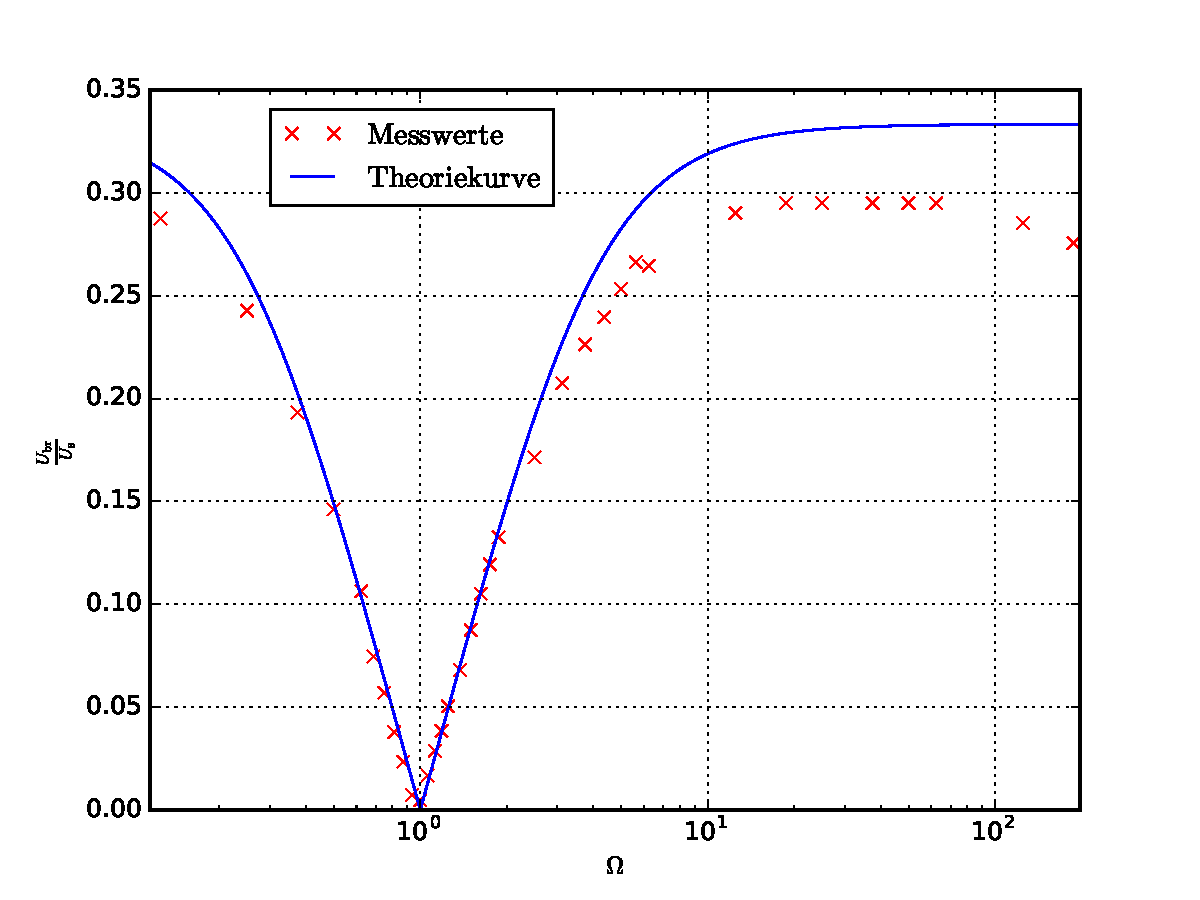
\includegraphics[width=1\textwidth]{pics/ub_us.pdf}
  \caption{Auftagung $\frac{\textfrak{U}\ua{br}}{\textfrak{U}\ua{s}}$  gegen $\Omega$ (halblogarithmisch) }
  \label{fig: plot}
\end{figure}

Wie in der der Vergrößerung der Abbildung \ref{fig: plot} zu sehen ist, erreicht die %ein der zu viel
Theoriekurve nie die Null.

\subsection{Bestimmung des Klirrfaktors}

Der Klirrfaktor wird mit \eqref{eq: klirr} bestimmt.
Wir nehmen dabei an das die Oberwelle nur aus der Spannung $U\ua{2}$ besteht. %an, dass
Dabei bestimmen wir $U\ua{2}$ mittels

\begin{equation*}
 U\ua{2}=U\ua{Br}\left(frac{1}{9} \frac{(\Omega^2 - 1)^2 }{(1 - \Omega ^2)^2 + 9 \Omega ^2}\right)^{-\frac{1}{2}}. %\frac
\end{equation*}

Zu Berechnung wir für $U\ua{Br}$ der minimale Wert $\textfrak{U}\ua{br\,min}$ %wird
genutzt und $\Omega=2$ gesetzt.
Für es ergibt sich der Wert %arrsch

\begin{equation*}
 U\ua{2}=\SI{0.005}{\volt}.
\end{equation*}
Die Abweichung liegt in der Größenordnung $\pm \, \SI{e-6}{\volt}$ und
wird nicht mit aufgeführt.
Um den Klirrfaktor zu bestimmen, nutzt man die gemittelte Speisespannung
$\overline{\textfrak{U}}\ua{s}=\SI{3.0\pm0.02}{\volt}$.
Damit resultiert für den Klirrfaktor der Wert:

\begin{equation*}
k=0.005
\end{equation*}
Der Fehler liegt in einer Größenordnung von $\num{e-6}$ und wird vernachlässigt.
